\documentclass[a4paper,11pt]{article}

\usepackage[greek,english]{babel}
\usepackage[utf8]{inputenc}

\newcommand{\lt}{\latintext}
\newcommand{\gt}{\greektext}

\usepackage{amsmath}
\usepackage[pdftex]{graphicx}
\usepackage{verbatim}
\usepackage[framed, numbered]{matlab-prettifier}

\usepackage{multirow}

\title{\gt Υποχρεωτική εργασία }
\author{\gt Όνοματεπώνυμο : \lt Kristi Cami \\ \gt ΑΕΜ: 3882}
\date{\gt Δεκέμβριος 29, 2021}

\begin{document}
    \maketitle
    \section{\gt Πρώτη Άσκηση}
    
        \begin{center}
             \begin{description}
                \item[(\gt α)] \textit {\gt {\small Να γίνει η γραφική παράσταση της παρακάτω συνάρτησης στο διάστημα  [0,3].}}
                
                \[ f(x) = 14xe^{x-2} -12e^{x-2} -7x^3 +20x^2 -26x +12 \]
                \begin{center}
                    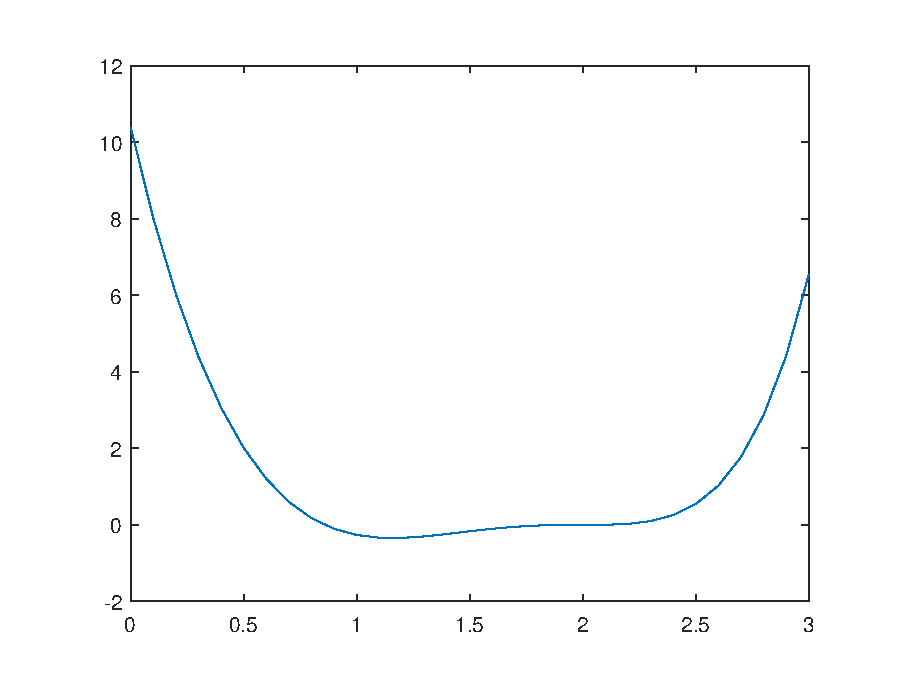
\includegraphics[width=.9\linewidth]{untitled.eps}\quad
                    \\[\baselineskip]
                \end{center}
                
                \textit {\gt {\small Όπως θα δούμε και θα αποδείξουμε παρακάτω η συνάρτηση έχει δυο ρίζες (2.00000 και 0.857114) στο διάστημα [0,3]. }}
                
                
                \newpage
                
                \item[(\gt β)] \textit {\gt {\small Υπολογισμός ριζών της συνάρτησης με την μέθοδο της διχοτόμησης σε \lt Matlab}}
                
                \vspace{5mm}
                
                \lstinputlisting[style=Matlab-editor]{ IntervalBisection.m}
                
                \begin{center}
                    \textit {\gt {\small Αποτελέσματα του παραπάνω προγράμματος}}
                    
                    \begin{center}
                        \begin{tabular}{ |l|l|l| }
                    
                            \hline
                            \gt Διάστημα & \gt Ρίζα &  \gt Επαναλήψης \\ \hline
                            \gt [0 , 1] & \gt 0.85714 &  \gt 53 \\ \hline
                            \gt [1 , 3] & \gt 2.00001 &  \gt 52 \\ \hline
                            
                
                        \end{tabular}
                    \end{center}
                    
                \end{center}
                
                \newpage
                
                \item[(\gt γ)] \textit {\gt {\small Υπολογισμός ριζών της συνάρτησης με τη μέθοδο \lt Newton-Raphson \gt σε \lt Matlab}}
                
                \vspace{5mm}
                
                \lstinputlisting[style=Matlab-editor]{ NewtonRaphson.m}
                
                \begin{center}
                    \textit {\gt {\small Αποτελέσματα του παραπάνω προγράμματος}}
                    
                    \begin{center}
                        \begin{tabular}{ |l|l|l| }
                    
                            \hline
                            \lt x0 & \gt Ρίζα &  \gt Επανάληψης  \\ \hline
                            \gt 0 & \gt 0.85714 &  \gt 7 \\ \hline
                            \gt 3 & \gt 2.00000 &  \gt 30 \\ \hline
                            
                
                        \end{tabular}
                    \end{center}
                    
                \end{center}
                
               
                    \textit {\gt {\small Παρατηρώντας τα αποτελέσματα καταλήγουμε στο συμπέρασμα ότι η ριζά 2.00000 δεν συγκλίνει τετραγωνικά διότι \lt f(2.00000)=0 \gt και \lt f'(2.00000)=0 \gt ενώ αντίθετα η ριζά 0.85714 συγκλίνει τετραγωνικά διότι ισχύει η συνθήκη \lt f(0.85714) = 0 \gt και \lt f'(0.85714) != 0. \gt Γενικότερα αν η \lt f(x) \gt δεν έχει συνεχή και φραγμένη πρώτη και δεύτερη παραγωγό, ή αν το αρχικό σημείο δεν είναι αρκετά κοντά στο σημείο μηδενισμού, τότε δεν έχουμε τετραγωνική σύγκληση.}}
                
                
                \newpage
                
                \item[(\gt δ)] \textit {\gt {\small Υπολογισμός ριζών της συνάρτησης με τη μέθοδο της τέμνουσας\gt σε \lt Matlab}}
                
                \vspace{5mm}
                
                \lstinputlisting[style=Matlab-editor]{ Secant.m}
                
                \begin{center}
                    \textit {\gt {\small Αποτελέσματα του παραπάνω προγράμματος}}
                    
                    \begin{center}
                        \begin{tabular}{ |l|l|l| }
                    
                            \hline
                            \gt Διάστημα & \gt Ρίζα &  \gt Επανάληψης\\ \hline
                            \gt [0 , 1] & \gt 0.85714 &  \gt 12 \\ \hline
                            \gt [2.5 , 3] & \gt 2.00000 &  \gt 41 \\ \hline
                            
                
                        \end{tabular}
                    \end{center}
                    
                \end{center}
            
                
            \end{description}
            
        \end{center}
        
    \newpage    
        
    \section{\gt Δεύτερη Άσκηση}
    
        \begin{description}
            \item[(\gt α)] \textit {\gt {\small \gt Τροποποιημένη μέθοδος \lt Newton-Raphson \gt με βάσει τον παρακάτω τύπο.}}
            
            \[ x_{n+1} = x_{n} - \frac{1}{\frac{f'(x_n)}{f(x_n)}-\frac{1}{2}\frac{f''(x_n)}{f'(x_n)}} \]
            
            \vspace{5mm}
            
            \lstinputlisting[style=Matlab-editor]{ ex2a.m}
            
            \newpage 
            
            \item[(\gt β)] \textit {\gt {\small \gt Τροποποιημένη μέθοδος διχοτόμησης οπού η εκτίμηση για την ριζά δεν είναι το μέσο του διαστήματος αναζήτησης σε κάθε βήμα αλλά ένα τυχαίο σημείο που επιλέγεται με την χρήση μια συνάρτησης \lt rand() \gt εντός του διαστήματος αναζήτησης}}
            
             \vspace{5mm}
            
            \lstinputlisting[style=Matlab-editor]{ ex2b.m}
            
             \newpage 
            
            \item[(\gt γ)] \textit {\gt {\small \gt Τροποποιημένη μέθοδος της τέμνουσας η οποία χεριάζετε 3 αρχικά σημεία και υπολογίζει την επόμενη εκτίμηση για την ριζά με βάση τον τύπο: }}
            
             \[ x_{n+3} = x_{n+2} - \frac{r(r-q)(x_{n+2} - x_{n+1} + (1-r)s(x_{n+2}-x_n)}{(q-1)(r-1)(s-1)} \]
             
             \textit {\gt {\small οπού }}
             
             \[ q=\frac{f(x_n)}{f(x_{n+1})} , r=\frac{f(x_{n+2})}{f(x_{n+1})} , s=\frac{f(x_{n+2})}{f(x_{n})} \]
             
             \textit {\gt {\small η μέθοδος αυτή είναι γνώστη και ως αντιστροφή τετραγωνική παρεμβολή. }}
             
             \vspace{5mm}
            
            \lstinputlisting[style=Matlab-editor]{ ex2g.m}
            
            \newpage
            
            \begin{enumerate}
                \item {\gt {\small Να βρεθούν όλες η ρίζες της παρακάτω συνάρτησης με ακρίβεια 5ου δεκαδικού ψηφίου στο διάστημα [-2,2] χρησιμοποιώντας της παραπάνω μεθόδους}}
                
                \[ f(x) = 54x^{6} + 45x^{5} - 102x^4 - 69x^3 + 16x + 4 \]
                
                \vspace{5mm}
                
                \begin{center}
                    \textit {\gt {\small \textbf{Αποτελέσματα τροποποιημένης \lt Newton-Raphson}}}
                    
                    \begin{center}
                        \begin{tabular}{ |l|l|l| }
                    
                            \hline
                            \lt x0 & \gt Ρίζα &  \gtΕπανάληψης  \\ \hline
                            \gt -2 & \gt -1.38129 &  \gt 5 \\ \hline
                            \gt -1 & \gt -0.66666 &  \gt 12 \\ \hline
                            \gt 0 & \gt 0.20518 &  \gt 4 \\ \hline
                            \gt 0.6 & \gt 0.50000 &  \gt 4 \\ \hline
                            \gt 1 & \gt 1.17611 &  \gt 5 \\ \hline
                            
                
                        \end{tabular}
                    \end{center}
                    
                \end{center}
                
                 \vspace{5mm}
                
                \begin{center}
                    \textit {\gt {\small \textbf{Αποτελέσματα τροποποιημένης μεθόδου διχοτόμησης }}}
                    
                    \begin{center}
                        \begin{tabular}{ |l|l|l| }
                    
                            \hline
                            \gt Διάστημα & \gt Ρίζα &  \gt Επανάληψης  \\ \hline
                            \gt [-2 , -1] & \gt -1.38129 &  \gt 69 \\ \hline
                            \gt  & \gt  &  \gt  \\ \hline
                            \gt [0 , 0.4] & \gt 0.20518 &  \gt 62 \\ \hline
                            \gt [0.4 , 1] & \gt 0.50000 &  \gt 74 \\ \hline
                            \gt [-2 , 2] & \gt 1.17611 &  \gt 68 \\ \hline
                            
                
                        \end{tabular}
                    \end{center}
                    
                    \textit {\gt {\small Παρατηρούμε ότι η μέθοδος αυτή χάνει μια ριζά την 0.66666}}
                    
                \end{center}
                
                
                \vspace{5mm}
                
                \begin{center}
                    \textit {\gt {\small \textbf{Αποτελέσματα τροποποιημένης μεθόδου τέμνουσας}}}
                    
                    \begin{center}
                        \begin{tabular}{ |l|l|l| }
                    
                            \hline
                            \lt x1 , x2 , x3 & \gt Ρίζα &  \gt Επανάληψης  \\ \hline
                            \gt -1.5 , -1.6 , 2 & \gt -1.38129 &  \gt 9 \\ \hline
                            \gt 0 , 1 , 2 & \gt -0.66666 &  \gt 17 \\ \hline
                            \gt -2 , 0 , 2 & \gt 0.20518 &  \gt 9 \\ \hline
                            \gt -1 , 1 , 2 & \gt 0.50000 &  \gt 11 \\ \hline
                            \gt 1 , 1.5 , 2 & \gt 1.17611 &  \gt 19 \\ \hline
                            
                
                        \end{tabular}
                    \end{center}
                    
                \end{center}
                
                \newpage
                
                \item {\gt {\small Εκτελώντας τον αλγόριθμο (β) 10 φορές παρατηρούμε ότι δεν συγκλίνει πάντα στον ίδιο αριθμό επαναλήψεων και αυτό οφείλετε στο γεγονός ότι η εκτίμηση για την ριζά επιλέγετε τυχαία από μια συνάρτηση παραγωγής τυχαίων αριθμόν}}
                
                \vspace{5mm}
                
                \item {\gt {\small Παρατηρούμε ότι η τροποποιημένη μέθοδο της διχοτομήσεις συγκλίνει ταχύτερα από την κανονική μέθοδο. Το ακριβός αντίθετο παρατηρούμε με της υπολείπεις δυο μεθόδους οπού η κανονικές συγκλίνουν ταχύτερα από της τροποποιούμενες.}}
                
            \end{enumerate}
            
     
        \end{description}
        
\end{document}